\usetikzlibrary{arrows}
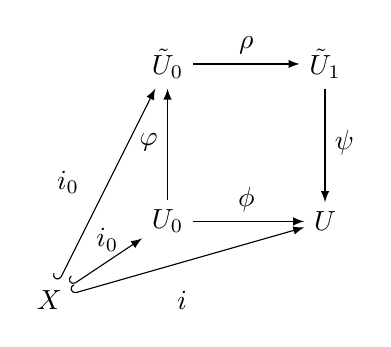
\begin{tikzpicture}

\node (v3) at (-1,1) {$U_0$};
\node (v2) at (1,1) {$U$};
\node (v1) at (-2.5,0) {$X$};

\node [above left] at (-1.5,0.5) {$i_0$};
\node [right] at (-1,0) {$i$};

\draw [-latex] (v3) edge (v2);
\draw[right hook -latex] (v1) edge (v2);
\draw [right hook -latex]  (v1) edge (v3);

\node [above] at (0,1) {$\phi$};

\node (U0') at (-1,3) {$\tilde{U}_0$};
\node (U1') at (1,3) {$\tilde{U}_1$};

\draw [-latex] (U0') edge (U1');

\node [above] at (0,3) {$\rho$};
%\draw [-latex] plot[smooth, tension=.7] coordinates {(-0.25,-0.5) (-2,0.5) (-2,2.5) (-1.25,3)};
\node [left] at (-2,1.5) {$i_0$};

\draw [-latex] (v3) edge (U0');
\node [left] at (-1,2) {$\varphi$};

\draw [-latex] (U1') edge (v2);
\node [right] at (1,2) {$\psi$};

\draw [right hook -latex] (v1) edge (U0');
\end{tikzpicture}